\chapter{Feedback and PID control}

In this lab you will be examining the effects of feedback on system
performance.  In particular, you will design a control, \(R_{C}\), for the
motor using the principles of PID control as shown in Figure~\ref{fig:PID}\@.
\begin{figure}[htbp]
    \centering
    \begin{picture}(300,75)
        \put(-1,50){\(\hat\theta_{d}(s)\)}
        \put(22,53){\vector(1,0){13}}
        \put(40,53){\circle{7}}
        \put(47,53){\vector(1,0){13}}
        \put(30,57){+}
        \put(30,43){\_}
        \put(63,37){\framebox(85,33){\normalsize\(P+I \frac{1}{s}+Ds\)}}
        \put(150,53){\vector(1,0){20}}
        \put(175,53){\circle{7}}
        \put(180,53){\vector(1,0){20}}
        \put(203,37){\framebox(42.5,33){\Large\(\frac{k_{E}}{s(s+\frac{1}{\tau})}\)}}
        \put(247,53){\vector(1,0){30}}
        \put(280,50){\(\hat\theta(s)\)}
        \put(259,53){\line(0,-1){45}}
        \put(259,8){\line(-1,0){219}}
        \put(40,8){\vector(0,1){40}}
        \put(180,58){\(\hat u(s)\)}
    \end{picture}
    \caption{PID control system}\label{fig:PID}
\end{figure}%

\section{Key Concepts}
In this lab, you will be implementing a PID controller into a closed loop
system. The main issue with open loop systems is that we only have
control over the reference trajectory, and therefore cannot account for
disturbances. Now, if we were to use feedback, we could attempt to control
the \emph{error} signal, which is the difference between the reference
trajectory (i.e.\ desired angle, or state of the motor) and the measured output.

A goal of a standard PID controller is to  tune the system to behave a certain
way by using various constants to correct the error signal. The three contstants
of a PID controller are \emph{Proportional}, \emph{Integral}, and \emph{Derivative}
controls.
\begin{itemize}
    \item \textbf{Proportional} control acts on the present value of the error signal. This is the most
          dominant of the three terms, but it can also leave some steady state error.
    \item\textbf{Integral} control accounts for the past values of error which is accumulated over time.
          This term will eliminate the steady state error that is left behind by the proportional control
          term, and also reduce rise time.
    \item \textbf{Derivative} control looks at the rate of change in the error signal, and attempts to
          correct for possible future values of error. For example, if the system is rapidly approaching
          its reference trajectory, (i.e.\ the error signal is rapidly approaching zero) the system will be
          able to slow down and avoid overshoot. Derivative control helps improve the settling time and
          stability of the system.
    \item Figure~\ref{fig:PIDExp} illustrates the concepts of a PID controller. You have some error
          signal, where the proportional term acts on the current state of the system, the integral term
          sums up all previous error, and the derivative term attempts to predict and control future error.

          \begin{figure}
              \centering
              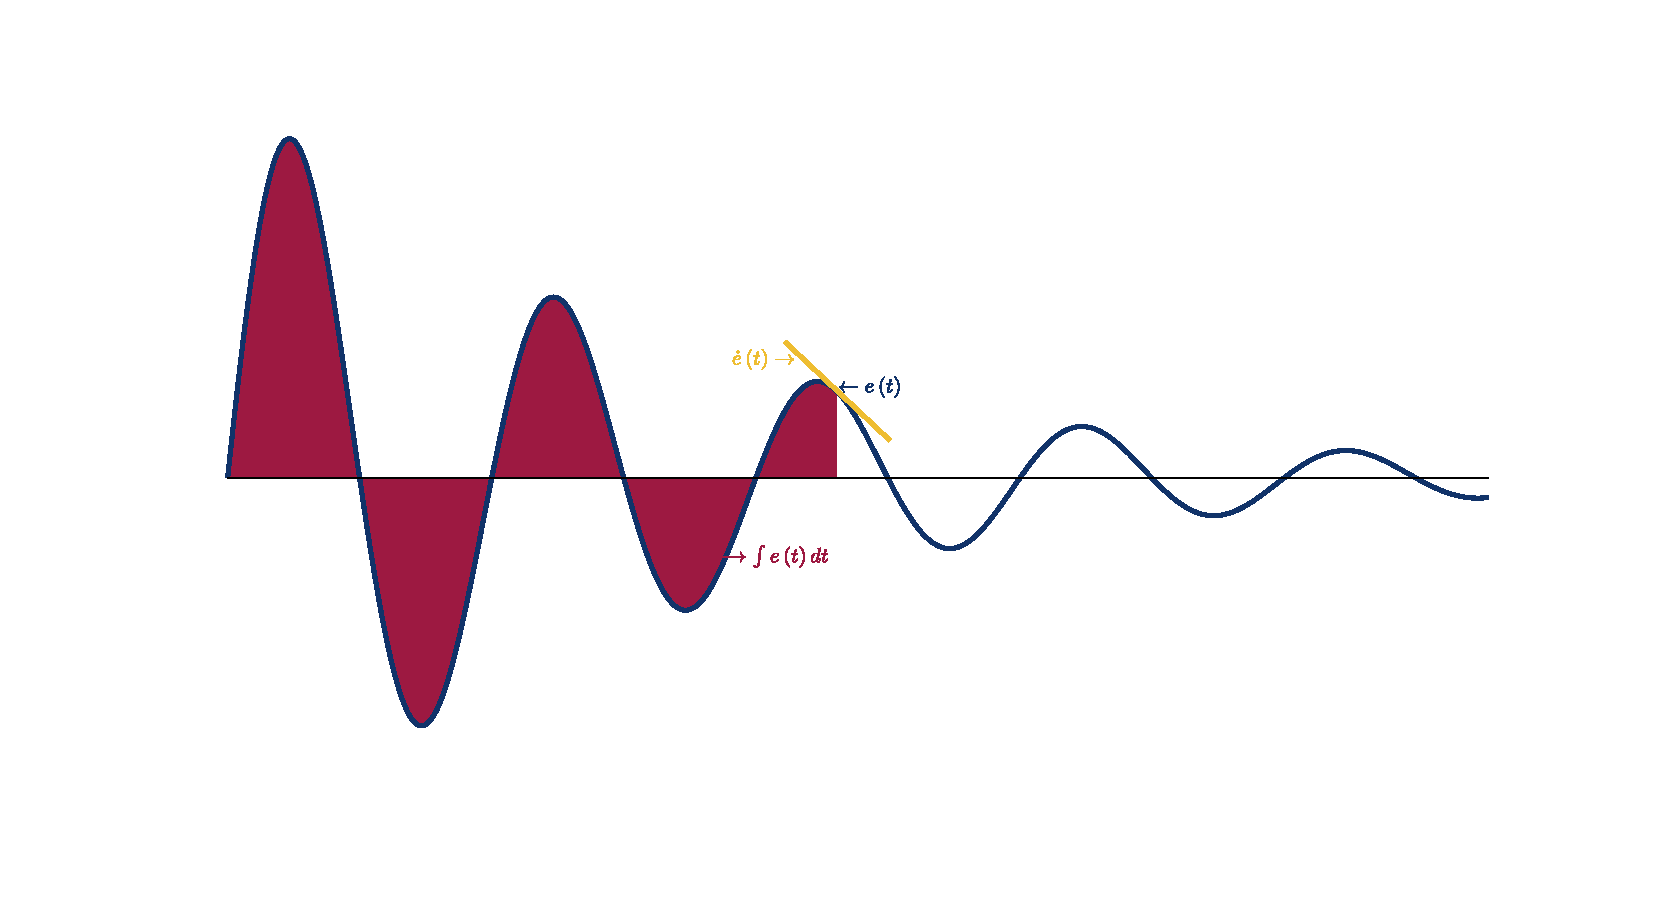
\includegraphics[width = 0.8\hsize]{pix/PIDSchematic.eps}
              \caption{Arbitrary error signal with a PID controller acting on it}\label{fig:PIDExp}
          \end{figure}

\end{itemize}
It is important to remember that when using  PID controllers, there will always be an element of
compromise within your system. For example, the ideal system will have a very low rise time, with
little to no steady state error or settling time, and no overshoot. However, this is very unrealistic in
the real world. If you were designing a highly precise robotic arm, you may need to tune your
controller in a way that there is practically no steady state error, but in order to do so, you will need to
have a higher rise time (i.e.\ the arm will move slowly, but it will go exactly where you need it). On
the other hand, you may have a system that requires a quick reaction time, for which you may need
to accept that there could be overshoot, or some steady state error.
\section{Prelab}

Before you go into the lab, you should read the following:
\begin{itemize}
    \item Sections 6.3 and 6.5 of the course notes.
    \item Learn the definitions for rise time, settling time, overshoot, steady-state value and steady state error.
\end{itemize}
Before the lab, complete the following steps:
\begin{enumerate}
    \item Using the Simulink model shown in Figure~\ref{fig:model6}, and identify
          the corresponding components from Figure~\ref{fig:PID}, i.e.\ what block acts as
          the plant, what is the reference trajectory, input, output, etc.
    \item Determine the closed loop transfer function.
    \item Determine the location of the closed loop poles when using P, I, D controls
          individually. What condition is required on the poles such that the system is BIBO stable?
\end{enumerate}

\section{Procedure}

\begin{enumerate}
    \item Prepare a \textsf{Simulink} model to implement a PID controller as
          shown in Figure~\ref{fig:model6}\@. \emph{Modify your model from lab 1 or 2}.
          \begin{figure}[htbp]
              \centering
              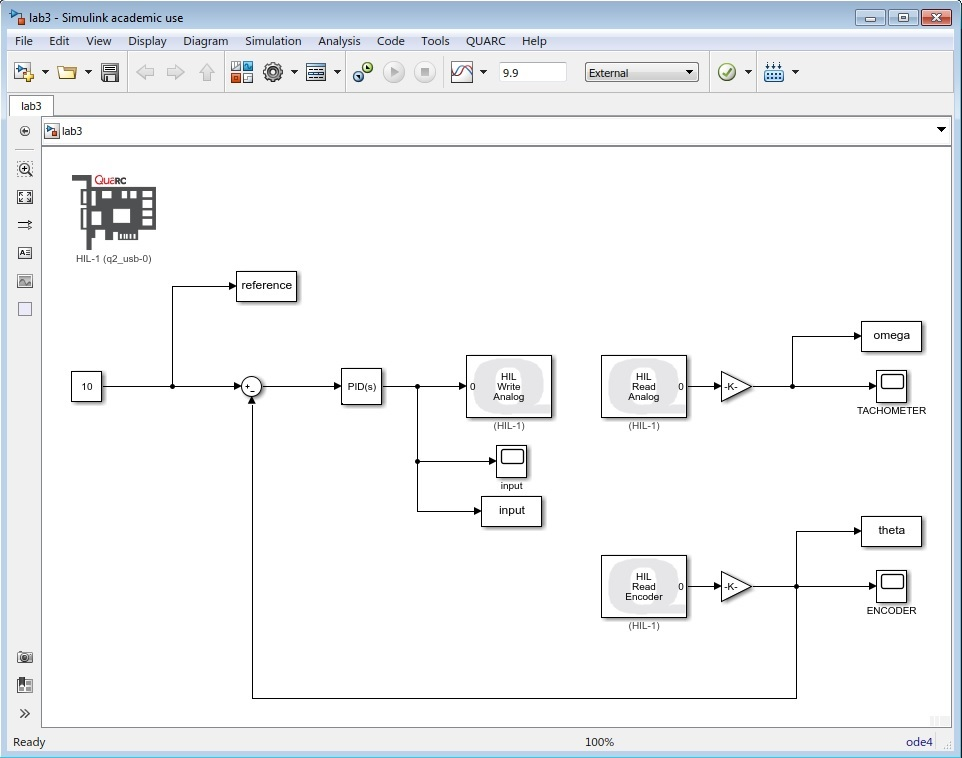
\includegraphics[width=0.6\hsize]{pix/lab3.jpg}
              \caption{\textsf{Simulink} model for the implementation of PID control}\label{fig:model6}
          \end{figure}%
          The \verb|PID| block can be found in the \verb|Simulink| menu under the
          \verb|Continuous| section parameters.

          As shown in Figure~\ref{fig:PIDparameters}\@,
          \begin{figure}[htbp]
              \centering
              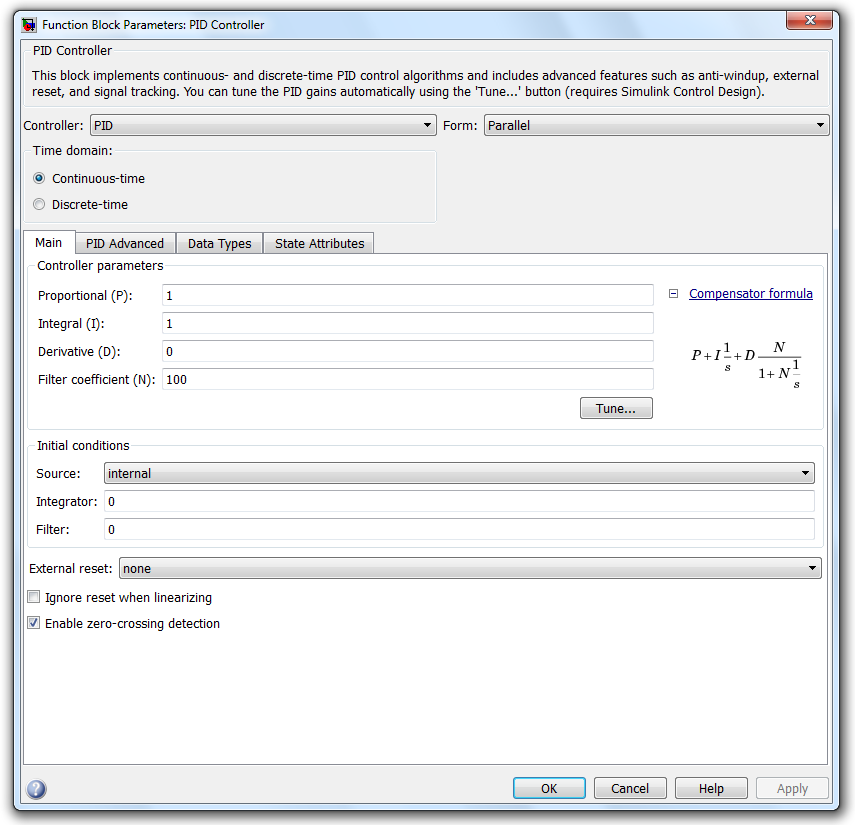
\includegraphics[width=0.6\hsize]{pix/PID.PNG}
              \caption{Screen shot of the \texttt{PID Controller} block}\label{fig:PIDparameters}
          \end{figure}%
          the \verb|PID| block contains three parameters: \(P\) is the proportional gain, of the controller; \(I\) is the integral action parameter which is equal; the \(D\) term provides the derivative action.
    \item\label{step:2} Set the desired angle to 10 radians.  The desired input is entered as
          shown in Figure~\ref{fig:model6} in the \verb|Constant| block. Remember to
          use the appropriate gain values from Table~\ref{tab:conversionFactors} for
          the encoder and tachometer to show results in radians.  Do not forget to
          change the \verb|solver| to \verb|ode 4| in \verb|Configuration Parameters|
          (\verb|Ctrl+E|).  Build and run the \textsf{Simulink} model using only the
          proportional term. Comment on the effects of using various values of \(P\).
          In particular, comment on the overshoot, rise time, settling time, and the
          steady-state error for different values of \(P\), and be sure to tabulate this data (a table in Excel is an efficient way to do this). Use at least three different values of \(P\).

    \item\label{step:3} Set \(D\) and \(I\) to 0 and increase the value of \(P\) so the
          system oscillates about the desired value of 10 radians without (seemingly)
          decreasing in magnitude. Print a copy of the encoder output at that value
          and print another plot with \(P\) having a value slightly less than this value.

    \item\label{step:4} Now reset your \(P\) value to the ``good'' value (i.e.\ not the value that makes
          the system oscillate about 10 radians, but the value where you get a ``desirable'' response). Test various \(D\) values while keeping \(P\) constant, and comment on overshoot, rise time, settling time, and steady-state error.
          Again, tabulate this data.

    \item\label{step:5} Decide on some satisfactory values of \(P\) and \(D\), and run the
          system again, using the integral control as well.  Comment on the overshoot,
          rise time, settling time, and steady-state error for various values of
          \(I\), and tabulate the data.

    \item Run the system using only the integral control term (i.e., set \(P\) and
          \(D\) to zero) and comment on the response of the system.  Using the
          transfer function, determine the roots of the characteristic polynomial.
          What insight does this give into the behaviour of the system using only
          integral control?

    \item We will now use a periodic saw-tooth function as our input.  To do
          this, replace the constant block by the block by the
          \verb|Repeating Sequence| block under the
          \verb|Simulink|\(\rightarrow \)\verb|Sources| menu.  The first parameter,
          \verb|Time Values|, indicates the switching times within one period.  The
          second parameter, \verb|Output Values|, indicate the values of the output of
          the block at the switching times considered.  So, for example, a saw-tooth of
          amplitude 1 and period 2 would have \verb|Time Values| set to \verb|[0 1 2]|
          and \verb|Output Values| set to \verb|[1 -1 1]|.

    \item Run the system with various combinations of proportional, integral, and
          derivative control.  Once you have a controller that tracks the input
          reasonably well, print a plot of the angle and the desired trajectory.

    \item Change the reference angle trajectory to add more switching times
          within a period.  To make things interesting, have the desired angle behave
          as four different functions on different intervals.  This can be achieved by
          preparing the \textsf{Simulink} model shown in Figure~\ref{fig:multiSwitch}\@.
          \emph{You do not need to use the exact same functions as shown in the figure}. Pick
          four functions that you think would be interesting.
          \begin{figure}[htbp]
              \centering
              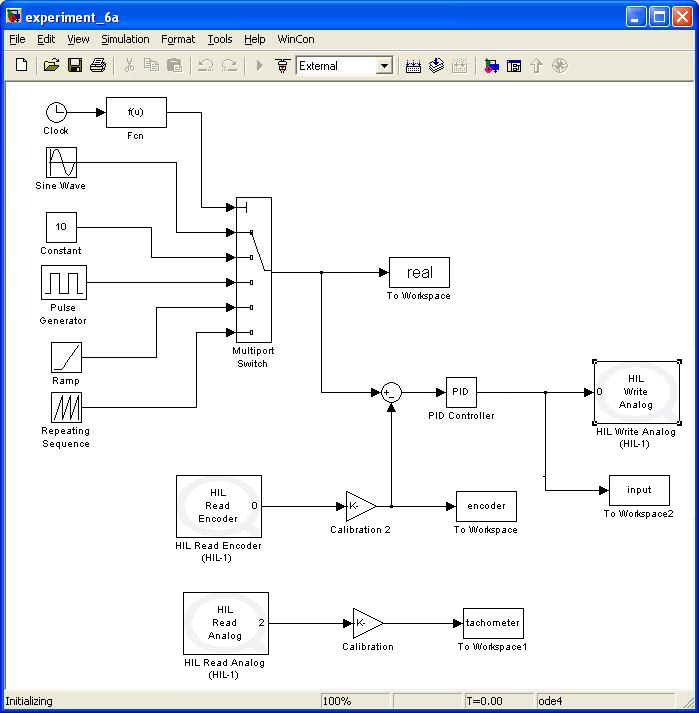
\includegraphics[width=0.6\hsize]{pix/lab6b.jpg}
              \caption{\textsf{Simulink} model for the implementation of multiple inputs and PID control}\label{fig:multiSwitch}
          \end{figure}%
          In this model, a number of possible sources have been introduced along with
          the switching logic.  The switching logic is based on the value of the
          function, \verb|4 sin(0.2*t)^{2}+1|.  This function, although arbitrary,
          assumes a value between 1 and 5 which is associated with ports 1 through 5 of
          the \verb|Multiport Switch| block.  The switching function is entered using
          the \verb|Fcn| block as indicated in Figure~\ref{fig:switchConfig}\@.
          \begin{figure}[htbp]
              \centering
              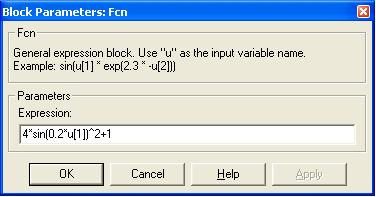
\includegraphics[width=0.6\hsize]{pix/fcnParameters.jpg}
              \caption{Configuration of the \texttt{Fcn} block for the implementation of multiple inputs and PID control}\label{fig:switchConfig}
          \end{figure}%

    \item Run the system and prepare a plot comparing the angle and the desired angle
          trajectory, making sure to note the values of the PID coefficients. You can
          reference Appendix~\ref{chap:hardware} for definitions of the previous
          concepts.

          When you have completed the lab, make sure you save your files in the folder
          you created in Lab~\ref{chap:intro}\@.

\end{enumerate}

\section{Deliverables}

Prepare a brief write up describing what you learned from this lab. This does not
need to be a formal report, but all material should be presented in a clear and logical manner,
with concise descriptions where necessary. Include the following / answer the following questions:
\begin{enumerate}
    \item Include tabulated data of the response characteristics from steps~\ref{step:2},~\ref{step:4}, and~\ref{step:5}.
          Be sure that you are using your ``good'' \(P\) value (i.e. NOT the value that makes the system oscillate about 10 rad / s) when collecting data for \(I\) and \(D\) tests.
    \item Comment on how varying \(P\), \(I\), and \(D\) values impact response characteristics (i.e.\ rise time, settling time, etc\ldots)
    \item Include the plot of the output that oscillates consistently about the reference trajectory of 10 radians
          generated in step~\ref{step:3}. Why do higher \(P\) values increase the oscillation of the output? What is
          happening to the location of the closed loop poles?
    \item Include the plot of the output when using only integral control. Using the transfer function, determine the roots
          of the characteristic polynomial.  What does this tell you about the behaviour of a system using only integral control?
    \item Include a plot of the output using your PID controller when the desired angle is generated by the multi-input
          switch. Be sure to specify your final P, I, and D values.
\end{enumerate}

%%% Local Variables: 
%%% mode: latex
%%% TeX-master: "lab-manual"
%%% End: 
